\documentclass{article}
\usepackage{graphicx} % Required for inserting images
\usepackage[utf8]{inputenc}
\usepackage[round]{natbib}
\usepackage{hyperref}
\usepackage[letterpaper, portrait, margin=1in]{geometry}
\usepackage{enumitem}
\usepackage{amsmath}
\usepackage{booktabs}
\usepackage{indentfirst}
\usepackage{float}
\usepackage{graphicx}
\usepackage{amsmath}
\usepackage{hyperref}
\hypersetup{
colorlinks=true,
    linkcolor=black,
    filecolor=black,      
    urlcolor=blue,
    citecolor=black,
}
\usepackage{natbib}
\usepackage{titlesec}
\titleformat{\section}
{\normalfont\Large\bfseries}{\thesection}{1em}{}[{\titlerule[0.8pt]}]

\title{ECON7103HHW06}
\author{sors3 Ors}
\date{February 2024}

\begin{document}

\maketitle

\section{Hourly data - Stata}

\begin{enumerate}
\item 
The number of treated cohorts is 539



\item 
the number of positive weights is 145467 and the negative weights is 48547


\item
Table \ref{tab:Q3} 1 shows the regression results of TWFE regression with hourly data. 

\begin{table}[ht]
    \centering
    \documentclass[]{article}
\setlength{\pdfpagewidth}{8.5in} \setlength{\pdfpageheight}{11in}
\begin{document}
\begin{tabular}{lc} \hline
 & (1) \\
VARIABLES & energy \\ \hline
 &  \\
treatment & -0.0434*** \\
 & (0.000232) \\
temperature & 0.00461*** \\
 & (1.21e-05) \\
precipitation & -0.000644 \\
 & (0.00200) \\
relativehumidity & 0.00230*** \\
 & (5.76e-06) \\
Constant & 0.539*** \\
 & (0.00111) \\
 &  \\
Observations & 720,000 \\
 R-squared & 0.664 \\ \hline
\multicolumn{2}{c}{ Robust standard errors in parentheses} \\
\multicolumn{2}{c}{ *** p$<$0.01, ** p$<$0.05, * p$<$0.1} \\
\end{tabular}
\end{document}

    \caption{TWFE hourly-data results}
    \label{tab:Q3}
\end{table}

\end{enumerate}


\section{Daily data - Stata}
\begin{enumerate}

\item 

Table \ref{tab: P2Q1} 2 indicates daily data results. To compare the hourly ATT and daily ATT, we may want to multiply hourly treatment by 24 and compare the results. 24*0.0434 = -10.416, which is very similar to the daily average treatment. Also, they are both significant. However, the reason for the difference can be the time of the treatment start. For example, the hours of the day can be different. 

\begin{table}[ht]
    \centering
    \documentclass[]{article}
\setlength{\pdfpagewidth}{8.5in} \setlength{\pdfpageheight}{11in}
\begin{document}
\begin{tabular}{lc} \hline
 & (1) \\
VARIABLES & energy \\ \hline
 &  \\
treatment & -0.936*** \\
 & (0.00557) \\
temperature & 0.111*** \\
 & (0.000379) \\
precipitation & 0.0681 \\
 & (0.188) \\
relativehumidity & 0.0552*** \\
 & (0.000189) \\
Constant & 12.88*** \\
 & (0.0341) \\
 &  \\
Observations & 30,000 \\
 R-squared & 0.972 \\ \hline
\multicolumn{2}{c}{ Robust standard errors in parentheses} \\
\multicolumn{2}{c}{ *** p$<$0.01, ** p$<$0.05, * p$<$0.1} \\
\end{tabular}
\end{document}

    \caption{TWFE daily-data results}
    \label{tab:P2Q1}
\end{table}

\item 
See Figure \ref{fig:P2Q1} 1
\begin{figure}[ht]
    \centering
    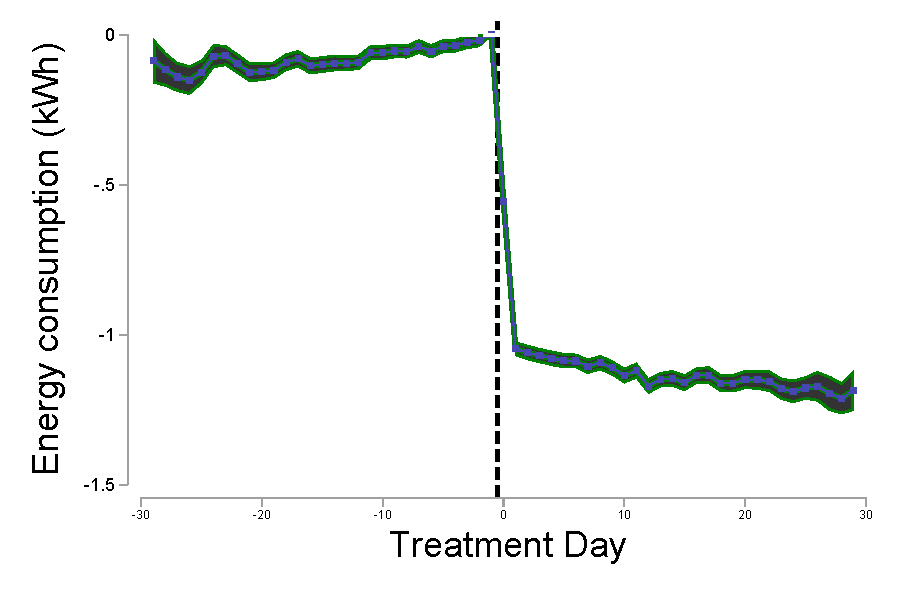
\includegraphics[scale = 0.7]{P2Graph1.pdf}
    \caption{Results with reghdfe}
    \label{fig:P2Q1}
\end{figure}


\item 
* I cannot run the result. It says that "command matsort is unrecognized". 
See Figure \ref{fig:P2Q2} 2
\begin{figure}[ht]
    \centering
    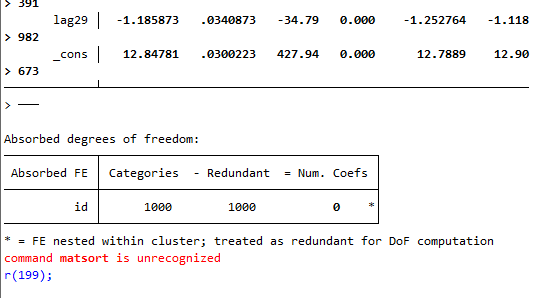
\includegraphics[scale = 0.7]{PSQ2.png}
    \caption{Results with eventdd}
    \label{fig:P2Q2}
\end{figure}

\item 
See Figure \ref{fig:P2Q3} 3
\begin{figure}[ht]
    \centering
    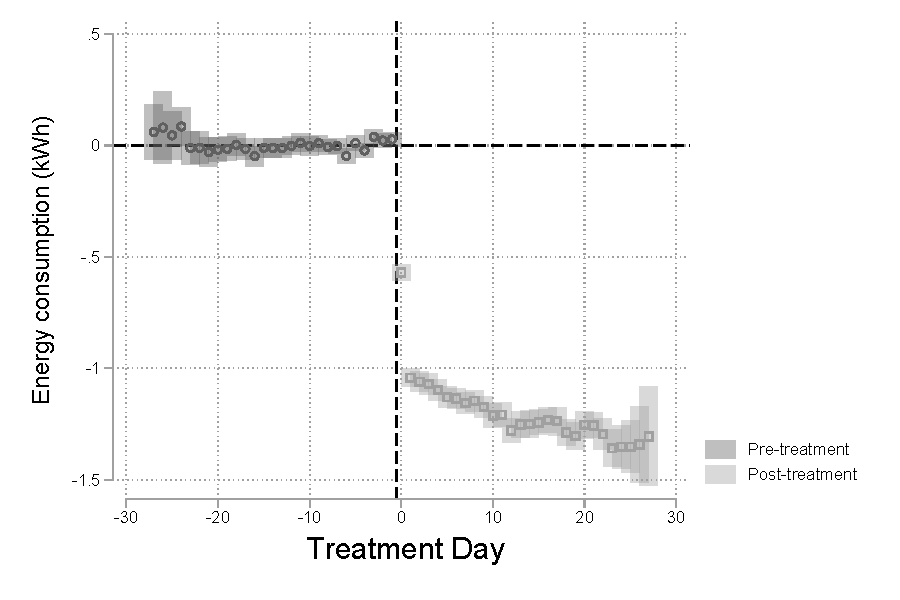
\includegraphics[scale = 0.7]{PSgraph3.pdf}
    \caption{Results with csdid}
    \label{fig:P2Q3}
\end{figure}


\end{enumerate}

\end{document}
